\PassOptionsToPackage{table}{xcolor}
\documentclass[nobib,nofonts]{tufte-handout}

%\geometry{showframe} % display margins for debugging page layout

%%% MF additions
% \usepackage[table]{xcolor}
\usepackage[nographicx, nohyperref, nosubcaption, nogb4e]{../99-auxiliary-files/00-mypackages}
\usepackage{../99-auxiliary-files/00-mycommands}
\usepackage{../99-auxiliary-files/00-myenvironments}

\addbibresource{~/Desktop/icloud/MyRefGlobal.bib}

\usepackage{titlesec}
\usepackage{etoolbox}
\usepackage{tikz-qtree}
\usepackage{subcaption}
\usepackage{CSPstyles}

\usepackage{pgfplots}
% externalize PGF plots
% \usepgfplotslibrary{external}
% \tikzexternalize

% \titleformat{\sectionj}
% {\large\bfshape}{\thesection}{1em}{}

\setcounter{secnumdepth}{5}
\renewcommand\thesection{\arabic{section}}

% this length controls tha hanging indent for titles
% change the value according to your needs
\newlength\titleindent
\setlength\titleindent{0.7cm}

\pretocmd{\paragraph}{\stepcounter{subsection}}{}{}
\pretocmd{\subparagraph}{\stepcounter{subsubsection}}{}{}

\titleformat{\chapter}[block]
  {\normalfont\huge\bfseries}{}{0pt}{\hspace*{-\titleindent}}

\titleformat{\section}
  {\normalfont\Large\itshape}{\llap{\parbox{\titleindent}{\thesection\hfill}}}{0em}{}

\titleformat{\subsection}
  {\normalfont\itshape}{\llap{\parbox{\titleindent}{\thesubsection\hfill}}}{0em}{}

\titleformat{\subsubsection}
  {\normalfont\normalsize\itshape}{\llap{\parbox{\titleindent}{\thesubsubsection}}}{0em}{}

\titleformat{\paragraph}[runin]
  {\normalfont\normalsize\itshape}{}{-0.7cm}{}[\xspace \ \ \ \ ]

\titleformat{\subparagraph}[runin]
  {\normalfont\normalsize}{\llap{\parbox{\titleindent}{\thesubsubsection\hfill}}}{0em}{}

\titlespacing*{\chapter}{0pt}{0pt}{20pt}
\titlespacing*{\subsubsection}{0pt}{3.25ex plus 1ex minus .2ex}{1.5ex plus .2ex}
\titlespacing*{\paragraph}{0pt}{3.25ex plus 1ex minus .2ex}{0em}
\titlespacing*{\subparagraph}{0pt}{3.25ex plus 1ex minus .2ex}{0em}

\DefineNamedColor{named}{mygray2}{cmyk}{0.55,0.25,0.25,0.25}
\newcommand{\mygray}[1]{\textcolor{mygray2}{#1}}

%%% Tufte style
\usepackage{graphicx} % allow embedded images
  \setkeys{Gin}{width=\linewidth,totalheight=\textheight,keepaspectratio}
  \graphicspath{{graphics/}} % set of paths to search for images

\usepackage{fancyvrb} % extended verbatim environments
  \fvset{fontsize=\normalsize}% default font size for fancy-verbatim environments

% Standardize command font styles and environments
\newcommand{\doccmd}[1]{\texttt{\textbackslash#1}}% command name -- adds backslash automatically
\newcommand{\docopt}[1]{\ensuremath{\langle}\textrm{\textit{#1}}\ensuremath{\rangle}}% optional command argument
\newcommand{\docarg}[1]{\textrm{\textit{#1}}}% (required) command argument
\newcommand{\docenv}[1]{\textsf{#1}}% environment name
\newcommand{\docpkg}[1]{\texttt{#1}}% package name
\newcommand{\doccls}[1]{\texttt{#1}}% document class name
\newcommand{\docclsopt}[1]{\texttt{#1}}% document class option name
\newenvironment{docspec}{\begin{quote}\noindent}{\end{quote}}% command specification environment

\newcommand{\proplog}{\acro{PropLog}}
\newcommand{\EFSQ}{\ensuremath{\mathit{EFSQ}}\xspace}

\renewcommand{\markdef}[1]{\emph{#1}}

\usepackage{pdfpages}

%%%%%%%%%%%%%%%%%%%%%%%%%%%%%%%%%%%%%%%%%%%%%%%%%%

% \usepackage[sc,osf]{mathpazo}
% \linespread{1.05}


\title[Relevant compression]{Relevance-guided information compression: \\ \Large{A primer on rate-distortion \& information-bottleneck theory}}

\author[M.~Franke]{Michael Franke, University of Tübingen}


\date{} % without \date command, current date is supplied

\begin{document}

\maketitle

\begin{abstract}
\noindent
Rate-distortion theory; information bottleneck theory; representation learning; communication; compression.
\end{abstract}

\noindent

\section{Relevance-guided information compression}

When acting in a complex environment, any agent, be it biological or synthetic, needs to process information about that environment in some way or other to achieve its goals.
But not all information in a vast world is equally relevant to the agent's concerns (whatever these may be: prediction, action-choice, reproductive success, \dots), and information processing will necessarily incur some resource costs (energy for fine-grained perception, representation, storage, \dots).
Consequently, two main factors influence information processing: the amount of relevant information processed (which is to be maximized) and the complexity of the information processing pipeline (which is to be minimized).
Clearly, these two factors are possibly conflicting constraints, so that any optimization of which and how much information to process for some ulterior goal must balance this \textbf{trade-off between representational economy and information relevance}.
This holds, in rudimentary form, for simple organisms optimized by natural selection, for more complex biological agents learning from their environment, and for artificial agents specifically designed by human engineers to learn statistical associations or action policies.

The trade-off between optimizing representational economy, on the one hand, and availability of relevant information, on the other hand, can be conceived of as a task of \textbf{relevance-guided information compression}.
Examples of such compression are clearest in engineering solutions such as the MP3 format which seeks to discard information in an audio file to reduce file size without sacrificing (too much) quality.
But the same trade-off also happens in cognition and communication.
For example, when forming concepts about the natural world at different levels of granularity (like \textit{animal}, \textit{dog}, \textit{poodle}), these can also be conceived as (near-)optimal solutions to the compression problem, with different weights for the competing forces of cutting and keeping information about relevant features and properties \citep{CorterGluck1992:Explaining-basi}.

\section{Information-theoretic models of relevant compression}

While cognitive systems are haunted by many different constraint-satisfaction problems \citep{Del-GiudiceCrespi2018:Basic-functiona}, the problem of relevance-guided information compression is addressed by two prominent frameworks couched in information theory.
One is rate-distortion theory (RDT), originally conceived by Claude Shannon, and another is a later extension of it, information-bottleneck theory (IB), introduced by \citet{TishbyPereira2000:The-information}.
Both frameworks are prominent as theoretical underpinnings in machine learning, relating especially to models for representation learning, such as autoencoders of different varieties.
They have also found applications in many areas of the cognitive (neuro-)sciences with contributions to, for example, perception \citep{Sims2016:Ratedistortion-,Sims2018:Efficient-codin}, memory \citep{Gershman2024:The-Rational-An}, or action choice \citep{LaiGershman2024:Human-decision-}.
The information bottleneck approach has gained prominence also in the language sciences where it can be used to explain the efficient coverage of meaning by a language's lexicon in a given semantic domain \citep[e.g.,][]{ZaslavskyKemp2018:Efficient-compr}.

RDT and IB are very similar in spirit, but also different in crucial conceptual detail.
We often encounter them in compact formulations as constraint-satisfaction problems, where their similarities and differences are not directly obvious.
The goal of this tutorial is to provide a deeper conceptual understanding of both and to highlight their similarities and differences.
For that reason, we do not begin by introducing RDT and IB in their usual (compact) ways formulations.
We begin by a high-level representation of the common problem that RDT and IB aspire to be solutions for, and then further elaborate on underlying assumptions, derivations and variations of both approaches.

\section{Actions or predictions from representations of partial observations}

We want a mechanism-agnostic model of an agent\sidenote{Speaking of an ``agent'' here is overly specific. The same optimality considerations would apply at a conceptual level, e.g., for a system that comprises distributed actors, such as a single signaling agent sending a message to a single receiver, or a whole population of senders and receivers (which may or may not be the same biological species), as long as we adopt the perspective of optimization for the \textit{whole} system.}
who receives (potentially partial) observations of their environment, represents these internally, and then acts on these internal representations.
The quality of the agent's actions or predictions depends on some state of the world, and the agent is able to adapt (and optimize for) which information they represent, and the way in which they respond to, or use, that represented information.

To model such a situation, we consider a \textbf{structure} $\mathcal{S} = \tuple{\mathcal{V}, P_{W}, \mathcal{L}}$, which fixes the unmutable background environment, and the agent's mutable \textbf{policies} $\mathcal{P}=\tuple{P_{E}, P_{D}}$.
The set $\mathcal{V}$ of (random) \textbf{variables} consists of: $X$ (observed part of the world state), $Y$ (unobserved part of the world state), $R$ (internal representation of $X$) and $O$ (some output, an action / prediction or similar formed based on $R$).
% More concretely, the state of world has two components: $X$ is the observable part (the input for the agent), $Y$ is what may have to recovered / predicted based on the information gleaned from $X$.
% The internal representation $R$ captures $X$ (or whatever is relevant from it) for decision making or prediction, and $O$ is the eventual output (choice, prediction, \dots) the agent makes (based on $R$).
The causal relations (and implied stochastic dependencies) of a structure and the policies are shown in Figure~\ref{fig:IB-RDT-dependencies}.
The variables $X$ and $Y$ are stochastically related in some way, as captured by the (ground-truth) joint probability distribution $P_{W}(X,Y)$.\sidenote[][-1.5cm]{For our current concerns, we need not know which of $X$ and $Y$ is causally downstream, or whether any stochastic dependency is due to a common cause. That's why Figure~\ref{fig:IB-RDT-dependencies} uses a special ``open-circle'' edge notation from work on ancestral causal graphs.}
The policies to be optimized consist of two parts: (i) the \textbf{encoder} is a conditional probability $P_{E}(R \mid X)$ assigning a probability over representations for each $x \in X$; and (ii) the \textbf{decoder} is a conditional probability function $P_{D}(O \mid R)$ assigning a probability over values of $O$ for each representation $r \in R$.
\marginnote{If $R$ is limited in its representational capacity, this creates a ``rate'' maximum for the information channel or an ``information-bottleneck.''}
Finally, the structure also fixes a \textbf{loss function} $\mathcal{L}$, which determines how successful any given trial was.
\marginnote{The main conceptual difference between RDT and IB is the loss function.}

We can unpack this by envisaging a sequential sampling \& scoring process (one sample from the environment/data and one iteration of encoding/decoding, resulting in a score for how good that trial was), which would proceed as follows:
\begin{align*}
  1. && (x,y) & \sim P_{W}(X,Y)    && \text{\textcolor{gray}{[sample from ground-truth, training or test data]}} \\
  2. && r & \sim P_{E}(R \mid X=x) && \text{\textcolor{gray}{[encode / represent the observed $x \in X$]}} \\
  3. && o & \sim P_{D}(O \mid R=r) && \text{\textcolor{gray}{[decode the representation / sample prediction]}} \\
  4. && \mathcal{L}(\cdot) & = \dots && \text{\textcolor{gray}{[score the trial by some numeric loss / inv.~utility]}}
\end{align*}
%
\begin{marginfigure}
  \centering
  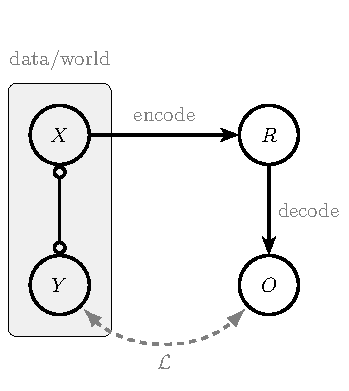
\includegraphics[]{00-pics/InfoBottleneck-RDT-causal-dependencies.pdf}
  \caption{Generalized common setup for RDT and IB. An observation of $X$ is encoded in representation $R$ and used to output $O$; the loss function depends on the output and the true $Y$.}
  \label{fig:IB-RDT-dependencies}
\end{marginfigure}
%
The full \textbf{joint distribution} over all four variables is therefore given by the factorization:
\begin{align*}
    & P(X=x,Y=y,R=r,O=o) \\
    & = P_{W}(X=x,Y=y) \times P_{E}(R=r \mid X=x) \times P_{D}(O=o \mid R=r)
\end{align*}
\marginnote{
  In the following, we mark the defining components of the full joint distribution with subscripts like $W$, $E$, and $D$.
  For all (marginal or conditional) probabilities that are derived from the joint distribution, we just write, e.g., $P(X \mid R)$ without any subscript.
}


\begin{remark}
  This setup is here formulated quite generally to showcase the applicability of both RDT and IB.
  Often RDT or IB are introduced based on setups that are special cases of the one laid out here (but many applications, especially of RDT, might consider more complex cases easily subsumed under the setup presented here).
  For example, the standard formulation of RDT, which textbooks might start out with \citep{ThomasCover1991:Elements-of-Inf}, considers the case where, intuitively speaking, ``$X=Y=O$,'' and the problem is framed as one of compression and reconstruction of the \textit{same} variable $X$.
  The formulation of IB actually requires the special case describable as ``$Y=O$,'' as the problem is conceived as that of matching the distribution of $O$ and $Y$ (see below).
  The more general formulation here, however, also allows the general perspective that relevance-guided information compression opens up.
  A signaling game without message costs (as studied in economics or biology), for instance, is also a special case of the setup shown above, describable as the case where ``$X=Y$.''
\end{remark}


\section{Formalizing representational economy}

Based on a scenario $\mathcal{S}$ and a pair of policies $\mathcal{P}$, we can give a more precise formulation of the problem of relevance-based information compression, which we conceive of as the trade-off between the maximization of information relevance, and the minimization of representational economy.

As for maximizing information relevance, the loss function $\mathcal{L}$ defines (indirectly) which pieces of information are comparatively more or less relevant.
We will see in more detail below that RDT and IB make different assumptions about the nature of the loss function (in a nutshell: scoring action policies or scoring beliefs / predictions), but the common idea is that $\mathcal{L}$ captures what matters to the agent's goals.

As for minimizing representational economy, this is where ideas from information theory come in.
While in any concrete system, considerations of physical / metabolic costs (e.g., for maintaining a perceptual or memory system, for producing and processing a signal, etc.) will play a role, from the point of view of a mechanism-agnostic, abstract, computational-level analysis, representational economy requires to minimize the \textit{amount of} information as such (no matter whether some physical system is better at storing \textit{this} type of information rather than \textit{that} type of information).
Since the information the agent can encode in principle in the assumed scenario is information about $X$ (their observations), the abstract requirement of representational economy adopted by RDT and IB is to minimize the mutual information $I(X,R)$ between the observations $X$ and $R$, which is defined as:
\begin{align*}
  I(X,R)
  & = \mathbb{E}_{(x,r) \sim P(X,R)} \log \frac{P(X=x, R=r)}{P(X=x) \times P(R=r)}
  % \\
  % & = \sum_{a,b} P(A=a,B=b) \times \log \frac{P(A=a, B=b)}{P(A=a) P(B=b)}
\end{align*}
Since in the given scenario, the joint distribution of $X$ and $R$ is factorized in terms of the (marginal) ground-truth probability of $X$ and the encoder's conditional probability of $R$ given $X$:
\begin{align*}
  P(X=x, R=r) = P_{W}(X=x) \times P_{E}(R=r \mid X=x)
\end{align*}
the representational economy constraint is entirely about the encoder and independent of the decoder.
Intuitively put, the mutual information between $X$ and $R$ is zero (which is the lowest possible value) if learning about $R$ doesn't tell you anything about $X$ and vice versa, i.e., that $X$ and $R$ are stochastically independent.
Reversely, the more information we can glean about $X$ given some $R$, the higher $I(X,R)$ becomes.
To even better understand this constraint, notice that we can rewrite mutual information in terms of  the entropy of $X$, $H(X)$, and the conditional entropy of $X$ given $R$, $H(X \mid R)$:
\begin{align*}
  I(X,R) & = H(X) - H(X \mid R) \\
  & = - \mathbb{E}_{x \sim P_{W}(X)} \log P_{W}(X=x) + \mathbb{E}_{(x,r) \sim P(X,R)} \log P(X=x \mid R=r)
\end{align*}
This reformulation shows how mutual information is a measure of the reduction of uncertainty about $X$ when learning $R$.
Figure~2 shows some examples of the interplay between the marginal probabilities $P(X)$, which govern $H(X)$, and the encoding policy.

In general, any encoding that is independent of $R$, i.e., that has $P(X \mid R=r_{i}) = P(X \mid R=r_{j})$, results in the minimum possible mutual information of 0 bits of information shared between variables.
In rough approximation, we can say that mutual information is maximized to the extent that the set of sets of observations $\set{x \in X \mid P(X=x \mid R=r) > 0}$ for each $r \in R$ is a partitioning of $X$ whose cells are as equally likely as possible.

\begin{figure*}[tp]
\renewcommand{\arraystretch}{1.05}
\setlength{\tabcolsep}{6pt}

\footnotesize

% ── subfigure (a) ──────────────────────────────────────────────────────────────
\begin{subfigure}[t]{0.48\linewidth}
\centering
\begin{tabular}{cccc}
\toprule
State & $P_{W}(X=x_{i})$ & $P_{E}(r_1\mid X=x_{i})$ & $P_{E}(r_2\mid X=x_{i})$ \\
\midrule
$x_1$ & $0.25$ & $1$ & $0$ \\
$x_2$ & $0.25$ & $1$ & $0$ \\
$x_3$ & $0.25$ & $1$ & $0$ \\
$x_4$ & $0.25$ & $1$ & $0$ \\
\bottomrule
\end{tabular}
\caption{$I(X,R) = 0$ bits}
\end{subfigure}
\hfill
% ── subfigure (b) ──────────────────────────────────────────────────────────────
\begin{subfigure}[t]{0.48\linewidth}
\centering
\begin{tabular}{cccc}
\toprule
State & $P_{W}(X=x_{i})$ & $P_{E}(r_1\mid X=x_{i})$ & $P_{E}(r_2\mid X=x_{i})$ \\
\midrule
$x_1$ & $0.25$ & $1$ & $0$ \\
$x_2$ & $0.25$ & $1$ & $0$ \\
$x_3$ & $0.25$ & $0$ & $1$ \\
$x_4$ & $0.25$ & $0$ & $1$ \\
\bottomrule
\end{tabular}
\caption{$I(X,R) = 1$ bit}
\end{subfigure}

\bigskip

% ── subfigure (c) ──────────────────────────────────────────────────────────────
\begin{subfigure}[t]{0.48\linewidth}
\centering
\begin{tabular}{cccc}
\toprule
State & $P_{W}(X=x_{i})$ & $P_{E}(r_1\mid X=x_{i})$ & $P_{E}(r_2\mid X=x_{i})$ \\
\midrule
$x_1$ & $0.25$ & $1$ & $0$ \\
$x_2$ & $0.25$ & $0$ & $1$ \\
$x_3$ & $0.25$ & $0$ & $1$ \\
$x_4$ & $0.25$ & $0$ & $1$ \\
\bottomrule
\end{tabular}
\caption{Suboptimal encoding: $I(X,R) = 0.8133$ bits}
\end{subfigure}
\hfill
% ── subfigure (d) ──────────────────────────────────────────────────────────────
\begin{subfigure}[t]{0.48\linewidth}
\centering
\begin{tabular}{cccc}
\toprule
State & $P_{W}(X=x_{i})$ & $P_{E}(r_1\mid X=x_{i})$ & $P_{E}(r_2\mid X=x_{i})$ \\
\midrule
$x_1$ & $0.55$ & $1$ & $0$ \\
$x_2$ & $0.15$ & $1$ & $0$ \\
$x_3$ & $0.15$ & $0$ & $1$ \\
$x_4$ & $0.15$ & $0$ & $1$ \\
\bottomrule
\end{tabular}
\caption{$I(X,R) = 0.7219$ bits}
\end{subfigure}


\bigskip

% ── subfigure (e) ──────────────────────────────────────────────────────────────
\begin{subfigure}[t]{0.48\linewidth}
\centering
\begin{tabular}{cccc}
\toprule
State & $P_{W}(X=x_{i})$ & $P_{E}(r_1\mid X=x_{i})$ & $P_{E}(r_2\mid X=x_{i})$ \\
\midrule
$x_1$ & $0.25$ & $0.8$ & $0.2$ \\
$x_2$ & $0.25$ & $0.8$ & $0.2$ \\
$x_3$ & $0.25$ & $0.2$ & $0.8$ \\
$x_4$ & $0.25$ & $0.2$ & $0.8$ \\
\bottomrule
\end{tabular}
\caption{$I(X,R) = 0.2781$ bits}
\end{subfigure}
\hfill
% ── subfigure (f) ──────────────────────────────────────────────────────────────
\begin{subfigure}[t]{0.48\linewidth}
\centering
\begin{tabular}{cccc}
\toprule
State & $P_{W}(X=x_{i})$ & $P_{E}(r_1\mid X=x_{i})$ & $P_{E}(r_2\mid X=x_{i})$ \\
\midrule
$x_1$ & $0.25$ & $0.8$ & $0.2$ \\
$x_2$ & $0.25$ & $0.7$ & $0.3$ \\
$x_3$ & $0.25$ & $0.3$ & $0.7$ \\
$x_4$ & $0.25$ & $0.2$ & $0.8$ \\
\bottomrule
\end{tabular}
\caption{$I(X,R) = 0.1984$ bit}
\end{subfigure}

\bigskip
\bigskip

\caption{
  Four encoder policies for $\card{X}=4$ and $\card{R}=2$.
  Each sub-table shows the marginal prior of each $x_{i}$ and the encoding strategy for that row.
}
\label{fig:mi-examples}
\end{figure*}


\section{Formalizing information relevance}

Both RDT and IB use the criterion of minimizing mutual information between $X$ and $R$ as a way of formalizing representational economy.
To implement the pressure towards a maximization of information relevance, the two approaches differ in their construal of the loss function $\mathcal{L}$.
In short, while RDT focuses on utility- or reward-based loss associated with actions and can be conceived of as a framework for policy learning, IB uses an information-theoretic loss function associated with probabilistic predictions and can be conceived of as a belief-learning approach.
Seen in this light, the difference between RDT and IB is similar to the difference between reinforcement learning (providing concrete reward signals based on physically realized actions) and belief-learning (where reward is based on the probability associated with a given event by the agent).
\marginnote[-2cm]{Roughly put: \\ RDT $\sim$ policy optimization \\ IB $\sim$ distribution matching}

The information relevance criterion for RDT is formulated in terms of a so-called \textbf{distortion function} $d \colon Y \times O \rightarrow \mathbb{R}$, which associates a loss, degree of deviation or inverse utility or reward with each pair of $Y$ and $O$.
The distortion function captures some kind of physical dissimilarity or practically relevant difference between $Y$ and $O$, similar to an (inverse) payoff function in reinforcement learning.
In the simplest case, which is also how RDT is usually first introduced, we consider the case describable as ``$X=Y=O$,'' so that the problem modelled is one of en- and decoding some variable $Y$ which is fully observed.
In that case the distortion function $d(y,y')$ would provide a measure of how close (in some practically relevant  sense) each pair of true $y$ and recovered $y'$ is.
But it is also possible, and not uncommon, to consider the more general case of including partial observations, and to even allow for the case where one variable $Y$ is encoded but the information is decoded into another variable $O$.
In the most general case, the \textbf{expected loss} of the whole system can be expressed as a function of the only mutable parts (the encoder and the decoder) in terms of the implied marginal distribution over $Y$ and $O$ as:
\begin{align*}
  \mathcal{L}(P_{E},P_{D}) = \mathbb{E}_{(y,o) \sim P(Y,O)} [d(y,o)]
\end{align*}

While RDT relies on a loss signal that is associated with (physical, practically relevant) differences between $Y$ and $O$, the IB approach is conceptually different, as it seeks to apply to cases where what needs to be learned is not an action policy as such, but a correct probabilistic prediction of $Y$.
Concretely, IB assumes that $O$ and $Y$ have the same range of values and relies on a loss function that enforces the minimization of information-theoretic surprisal, which can be stated as the requirement that the agent (the pair of encoder and decoder policies) should minimize the cross-entropy between $Y$ and $O$:
\begin{align*}
  \mathcal{L}(Y,O) & = \text{CE}(Y,O) \\
  & = - \mathbb{E}_{y \sim P(Y)} \log P(O=y)
\end{align*}
The cross-entropy loss between a ground-truth distribution like $P(Y)$ and a predicted output distribution $P(O)$ is common for belief-learning setups.
However, the usual formulation of the IB objective is not in terms of cross-entropy but in terms of mutual information.
However, we can \emph{derive} the usual mutual information-based formulation of IB's information relevance from this cross-entropy loss function, and in doing so see that:
\begin{itemize}
  \item the belief-learning approach of IB in terms of information-theoretic loss is conceptually different from the pure outcome-based loss of RDT in the sense that the former, but not the latter, requires the agent to track the probability of its own output predictions;
  \item minimizing cross-entropy loss entails a simple functional form for the decoder (namely standard Bayesian posteriors), so that we can focus entirely on the encoder part of the policies.
\end{itemize}


The cross-entropy loss can be rewritten in terms of a conditional entropy that depends on the encoder only, and a requirement to minimize the KL-divergence between the posterior $P(Y \mid R)$ and the encoder $P_{D}(O \mid R)$:
\begin{align*}
  \mathcal{L}(Y,O)
  & = - \mathbb{E}_{y \sim P(Y)} \log P(O=y)
  \\
  & = - \mathbb{E}_{(y,r) \sim P(Y,R)} \log P_{D}(O=y \mid R=r)
  \\
  & = \mathbb{E}_{(y,r) \sim P(Y,R)} - \log P_{D}(O=y \mid R=r)
  \\
  & = \mathbb{E}_{(y,r) \sim P(Y,R)} [- \log P_{D}(O=y \mid R=r) + \underbrace{\log P(Y=y \mid R=r) - \log P(Y=y \mid R=r)}_{=0 \text{\ \ for all} y, r}]
  \\
  & = \mathbb{E}_{(y,r) \sim P(Y,R)} - \log P(Y=y \mid R=r) + \mathbb{E}_{(y,r) \sim P(Y,R)} \frac{\log P(Y=y \mid R=r)}{\log P_{D}(O=y \mid R=r)}
  \\
  & = \underbrace{\text{H}(Y \mid R)}_{\text{conditional entropy}} + \underbrace{\text{KL}[P(Y \mid R)\, ||\, P_{D}(O \mid R)]}_{\text{Kullback-Leibler divergence}}
\end{align*}

Notice that the latter KL-term is minimized whenever the decoder implements the Bayesian posterior $P(Y \mid R)$ precisely.
For this reason, when we are only interested in the theoretical optimal solution to the optimization problem, it may suffice to focus on the encoder $P_{E}$ and assume throughout that the decoder \textit{is} given by Bayes rule.
\marginnote{In non-idealized situations, e.g., where encoder and decoder are implemented via approximate function learning modules (e.g., neural networks), similar consideration lead to variational approaches to IB.}

The former term $H(Y \mid R)$ is independent of the decoder, but directly relates to mutual information because:
\begin{align*}
  I(Y,R) = H(Y) - H(Y \mid R)
\end{align*}
Since $H(Y)$ is a constant independent of the encoder or decoder, the objective to minimize cross-entropy can be reduced, assuming ideal conditions, to the requirement to minimize $I(Y,R)$.

The original formulation in terms of a cross-entropy loss has the advantage of showing the parallel to belief-learning frameworks and to highlight that, even though a formulation in terms of $I(Y,R)$ suggests a global-distributional objective, agents can optimize their own encoder and decoder policies based on a sampling-based approximation of the cross-entropy loss, as long as they have access to the point-wise probability $P(O=y \mid Y=y)$ entailed by their policies.

\section{Optimal trade-offs in RDT \& IB}

The optimization of representational economy and information relevance is non-trivial, because the more we optimize one, the worse we are off with the other.
In generally, whenever two objectives $A$ and $B$ are inversely proportional, we may have infinitely many \textbf{Pareto-optimal solutions}, in the sense that we cannot get better for $A$ without getting worse for $B$ and vice versa.
This also holds for IB in general, and it holds for RDT under most practically relevant distortion functions.
Consequently, the optimization problem is usually formulated as one where we optimize $A$ under the requirement that $B$ may not be worse than a particular fixed value (or, equivalently, the other way around).
This then entails an \textbf{optimality frontier}, or \textbf{Pareto frontier}, the line of optimal solutions when fixing an desirable upper-bound for representational complexity or loss, as stylistically shown for IB in Figure~\ref{fig:Pareto-curve}.
This line splits the set of possible values for representational complexity and loss into two regimes: the possible, non-optimal but realizable values; and the ``super-optimal'' values that are mathematically impossible to achieve given the conflicting forces of representational complexity and loss.

\begin{marginfigure}
  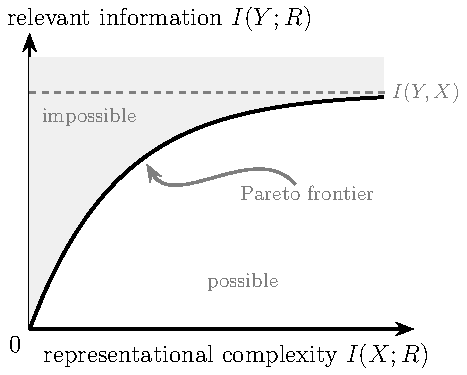
\includegraphics[]{00-pics/InfoBottleneck-RDT-Pareto-curve.pdf}
  \caption{Stylized Pareto-frontier for IB. We want to be as far left and up as possible. But at the Pareto-frontier we cannot optimize in either direction, without getting worse on the other. Relevant information is theoretically capped at $I(X,Y)$, which in turn is capped at $H(Y)$.}
  \label{fig:Pareto-curve}
\end{marginfigure}

Another way of looking a constraint-satisfaction problem in general, and the trade-off between representational economy and information relevance in particular, is to zoom in on the fact that we cannot determine a simple and \textit{single best} solution unless we decide on how to weigh the conflicting components.
Suppose that my agent is currently in a state where $A=3$ and $B=2$.
You propose a deal so that I can sacrifice two units of $A$ for one unit of $B$.
If I accept the deal, my agent would be in the state where $A'=5$ and $B'=1$.
Should I take that deal?
Is the new state better, the same or worse than the old? ---
That depends on how one unit of $A$ is weighed against one unit of $B$, of course.
This is why the dual objectives of RDT and IB are often very compactly stated in terms of loss function that contains a \textbf{trade-off parameter} $\beta$ weighing the representational complexity term (or inversely: the amount of compression), formulated as the mutual information between input $X$ and its encoding representation $R$, and an inverse utility, reward, or accuracy term spelled out in terms of a distortion function $d$ or IB's measure of relevant information in terms of mutual information $I(Y,R)$:
\begin{align*}
  \mathcal{L}_{\text{RDT}} & = \underbrace{I(X,R)}_{\text{compression}} + \beta \ \underbrace{\mathbb{E}_{(y,o) \sim P(Y,O)} [ d(y,o) ]}_{\text{distortion (reconstruction loss)}} \\
  \mathcal{L}_{\text{IB}}  & = \underbrace{I(X,R)}_{\text{compression}} - \beta \ \underbrace{I(Y,R)}_{\text{relevant information}}
\end{align*}




\newpage

\printbibliography

\end{document}

